% fundDom.tex      pdflatex ZhCvGo15

% Diffuse globally, compute locally: a cyclist tale
% Tingnan Zhang, Daniel I. Goldman and Predrag Cvitanovi\'c

%\section{Into the fundamental domain}
%\label{s-fundDom}

%\begin{figure}[htbp]
%  \begin{center}
%    (a)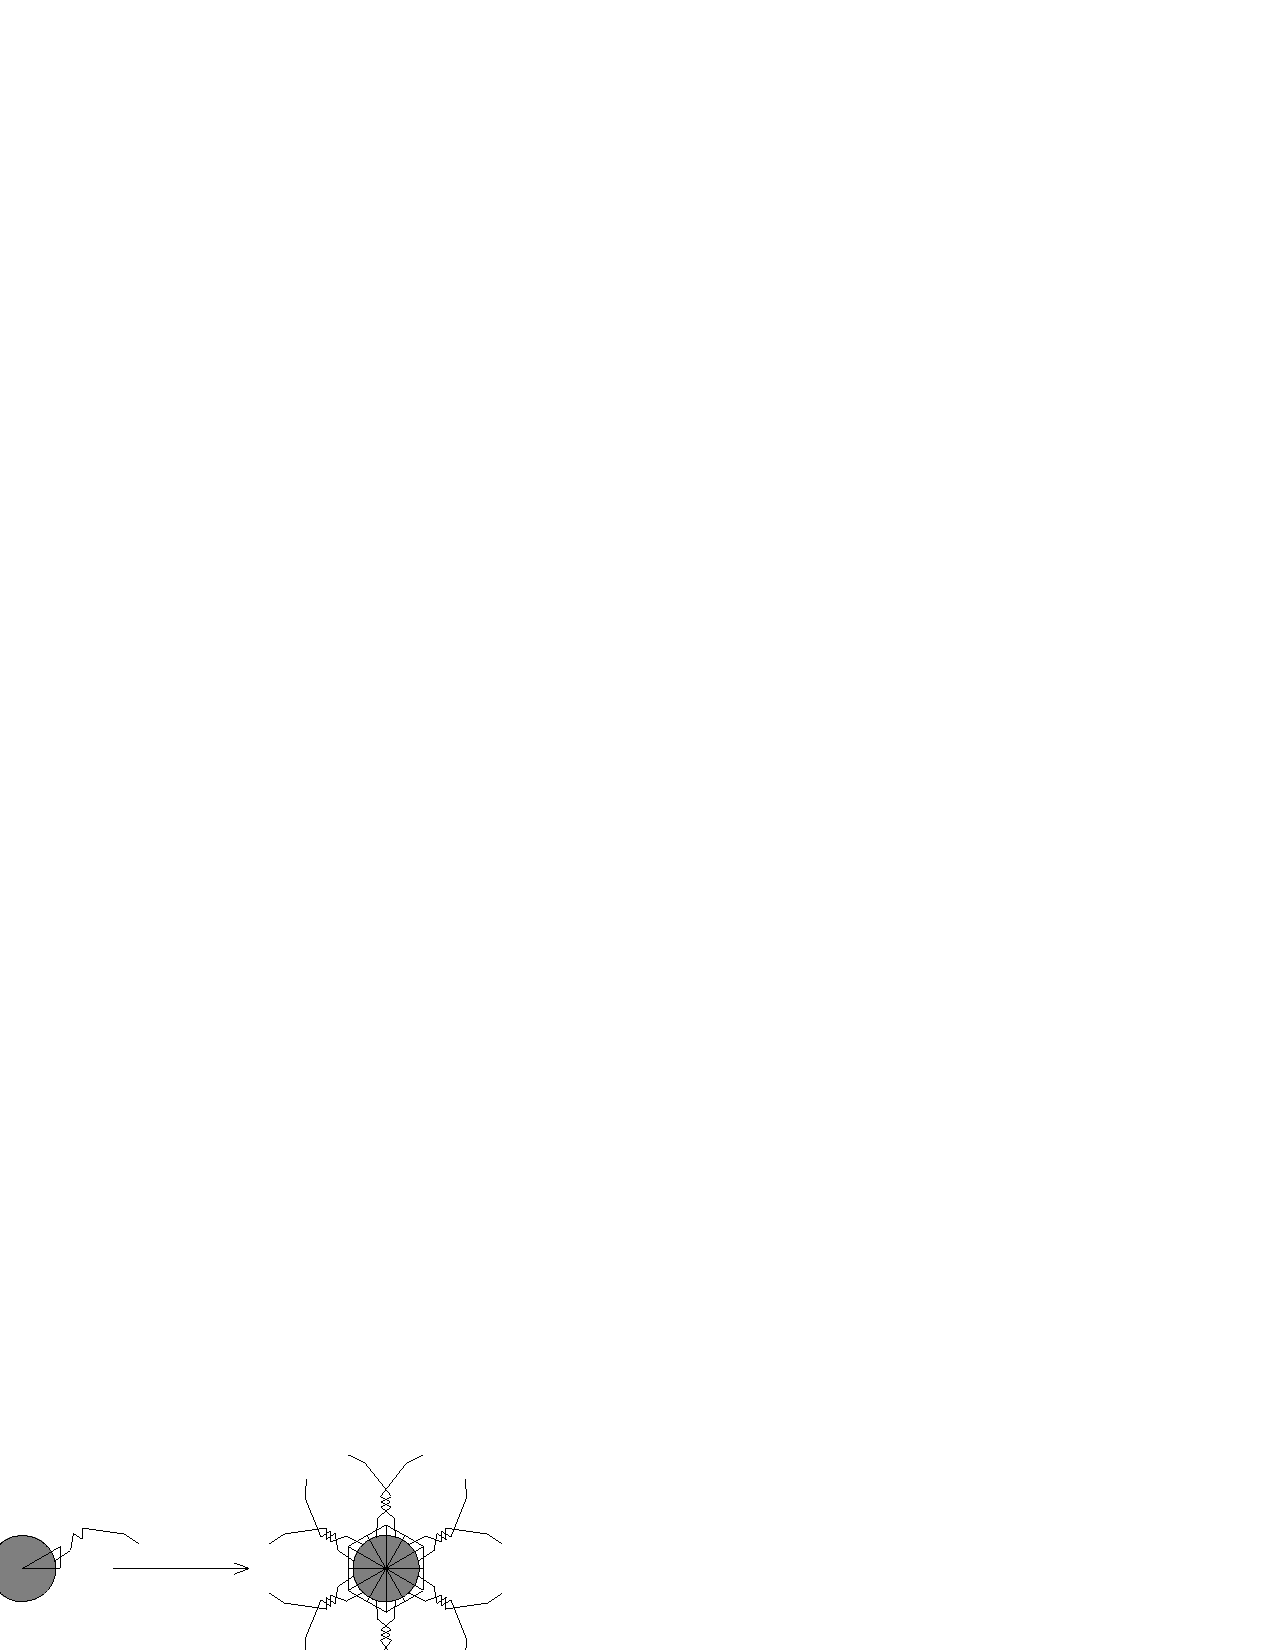
\includegraphics[width=0.45\textwidth]{diffuseSchreiberFig2}
%    (b)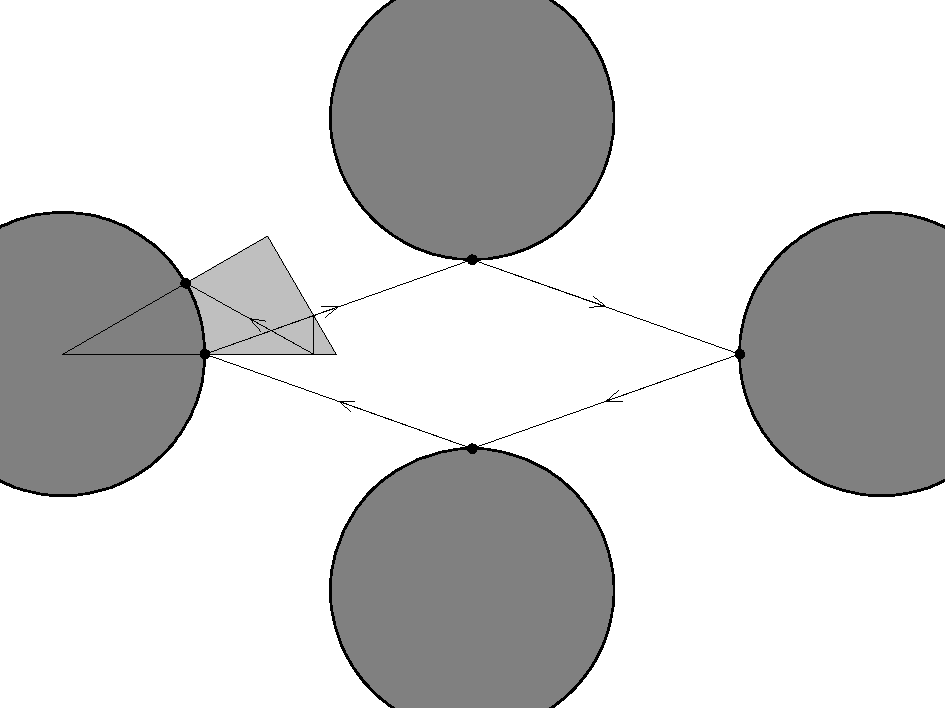
\includegraphics[width=0.45\textwidth]{diffuseSchreiberFig3}
%  \end{center}
%  \caption[]{ \label{fig:schrieberFig23} (a) An (unwrapped) trajectory (in full
%  space) and its 12 copies after applying point group actions to it. (b)
%  Multiplicity of periodic orbits in fundamental domain.}
%\end{figure}

%When the scattering array has a discrete symmetries, such as
%reflection symmetry, each elementary cell may be built from a {\em
%fundamental domain} ${\widetilde \pS}$ by the action of a discrete (not
%necessarily abelian) group $G$. The quantity $\tx(t)\,=\,\tflow{t}{\tx}$
%denotes the flow in the fundamental domain ${\widetilde \pS}$;
%$\tflow{t}{\tx}$ is related to$\flow{}{\tx}$ by a discrete symmetry $g
%\in G$ which maps $\tx(t)\in{\widetilde \pS}$ to ${x}(t) \in {\pS}$. The
%full $\hM \rightarrow {\widetilde\pS}$ reduction is complicated by the
%non-abelian nature of $G$, and will be illustrated in this section in
%detail.

In \refref{LorentzDiff} some effort, unsuccessful, was made to derive a
diffusion formula for the fully symmetry-reduced dynamics, involving only
quantities computed within the fundamental domain. The fact that lattice
translations do not commute with the symmetry group within the elementary
cell makes this apparently a difficult task. The main achievement of this
paper is a new proposal how to extend \po\ theory in order to solve this
vexing problem.

In \refsect{s-Lorentz} we had
reduced a trajectory from full space to elementary cell, as in
\reffig{fig-schrieberFig12}\,(a), upper right, using the translational
symmetry, and were able to compute various quantities in terms of
elementary cell \po s. In this section we will further utilize the
point group symmetry to derive the fully symmetry-reduced trace
formula and, for the first time, the diffusion constant using cycles
restricted to the fundamental domain.


\subsection{Point group changes translation \label{s-FundTranslation}}

A point $\ssp$ in the elementary cell is identified by its
fundamental domain mirror image:
\[ %beq
\ssp=g\,\tx,
\] %eeq
given a little group action $g\in G$. We have to appreciate that both
the full space flow $\hflow{t}{\ssp}$ and elementary flow
$\flow{t}{\ssp} $ is G-equivariant under the lattice group symmetry,.
\beq
\hflow{t}{g\,\tx} = g\,\hflow{t}{\tx}\,,
\flow{t}{g\,\tx} = g\,\flow{t}{\tx}\,,
\label{eq-equivariance-flow}
\eeq

It follows that the displacement in full space is also G-equivariant
under the little group:
\beq
\hn_t(\ssp) = \hflow{t}{g\,\tx} - \flow{t}{g\,\tx}
            = g\,(\hflow{t}{\tx} - \flow{t}{\tx})
            = g\,\hn_t(\tx)\,.
\label{eq-equivariance-disp}
\eeq
However, this nice property does not automatically resolve the problem
at hand. When the dynamics is restricted to the fundamental domain,
we lose the absolute orientation. We show this
by following a prime \po\ $\tp$ in the fundamental domain.

Let $\tp\equiv\{\tx_1,\ldots,\tx_{\cl{\tp}}\}$, with topological length
$\cl{\tp}$ and $\tx_i$ the points of collision on the orbit. Starting
from the edge of disk at $\tx_i$, at some point the flight will meet one
of the triangle boundaries of the fundamental domain and be deflected
back. In the full space the particle continues to another triangular
domain, which, in general, does not have the same orientation to the
original copy (figure here). The relative change in the orientation can
always be described by a element of the little group. Before the particle
reaches the next collision point $\tx_{i+1}$, it has crossed multiple
boundaries (or symmetry lines), and we denote the accumulated change in the
orientation by $g_\tp(\tx_{i},\tx_{i+1})$.

Denote the displacement of flight $(\tx_i, \tx_{i+1})$ as
$\hn_{\tp}(\tx_i, \tx_{i+1})$, the added displacement from
$\tx_i$ to $\tx_{i+2}$ is
\beq
    \hn_{\tp}(\tx_i, \tx_{i+2}) = \hn_{\tp}(\tx_i, \tx_{i+1}) +
    g_\tp(\tx_{i}, \tx_{i+1})\hn_{\tp}(\tx_{i+1}, \tx_{i+2})\,,
\eeq
\ie, we have to memorize the change in the relative orientation.
Applying this rule to the entire cycle, we have (after applying a
cyclic shift $\cl{\tp} + 1 \to 1$)
\beq
\hn_{\tp}(\tx_{1})=\sum_{i=1}^{\cl{\tp}}g_{\tp}(\tx_{1},
\tx_{i})\,\hn(\tx_{i}, \tx_{i+1}),
\eeq
where the left order product $g_{\tp}(\tx_{1},
\tx_i)=\prod_{j=1}^{i-1} g_\tp(\tx_{j},\tx_{j+1})$, and
$g_{\tp}(\tx_1, \tx_1) = e$. Unlike in the elementary cell, the
displacement in general is dependent on the starting point.
%\beq
%\hn_{\tp}(\tx_2) = g_{\tp}^{-1}(\tx_1, \tx_2)(\hn_{\tp}(\tx_{1}) -
%\hn_{\tp}(\tx_1, \tx_2)) + h_{\tp}(\tx_1)\hn_{\tp}(\tx_1, \tx_2)
%\eeq
We define the total group action (orientation change) for the orbit
\beq
h_{\tp}(\tx_1)=\prod_{i=1}^{\cl{\tp}}
g_\tp(\tx_{i},\tx_{i+1})\,,
\label{eq-cyclegrp-fd}
\eeq
which immediately connects the flow in fundamental domain and
elementary cell by
\beq
\flow{t_\tp}{\tx_i}=h_{\tp}(\tx_i)\tflow{t_\tp}{\tx_i}\,.
\eeq

Although the group action $h_{\tp}(\tx_i)$ depends on the initial
points on the orbit as well, it is a property of the orbit's
symmetry. Using \refeq{eq-cyclegrp-fd}, one can easily show that all 
$h_{\tp}(\tx_i), \tx_i\in\tp$ belong to the \emph{same} subgroup of $G$


\beq
h_{\tp}(\tx_{i+1}) = g_{\tp}^{-1}(\tx_i, \tx_{i+1})\,
h_{\tp}(\tx_{i})\,g_{\tp}(\tx_i, \tx_{i+1})\,.
\eeq
If we let the particle (starting from $\tx_i$) travel along the
fundamental domain orbit $r$ times, the result displacement is
\beq
\hat{L}_{\tp}(r, \tx_i)\equiv
(e+\hp^{1}(\tx_i)+\cdots+\hp^{r-1}(\tx_i))\cdot\hn_{\tp}(\tx_i)\,.
\label{eq-fd-displacement}
\eeq
